\documentclass[10pt, a4paper]{article}

\usepackage{ctex}
\usepackage{xeCJK}
\usepackage{caption}
\usepackage{geometry}
\geometry{
    left = 0.6in,
    right = 0.6in,
    top = 0.8in,
    bottom = .6in
}
\usepackage{amssymb}
\usepackage{amsbsy}
\usepackage{amsmath}
\usepackage{xcolor}
\usepackage{mathrsfs}
\usepackage{graphicx}
\usepackage{pifont}
\usepackage{tikz}
\usepackage{tasks}
\settasks{
    label = \textcolor{purple}{\Alph*.},
    label-width = 14pt
}
\pagestyle{empty}

\newcommand{\Title}[3]{
    \begin{center}
        \Large \textbf{中国电子学会 #1~年~#2~月 Scratch~#3级考试}
    \end{center}
}
\newcommand{\TimeAndName}[1]{
    \begin{center}
        考试时间:~#1~ 分钟 \qquad\qquad\qquad\qquad 姓名:\underline{\quad\quad\quad\quad}
    \end{center}
}
\newcommand{\hq}{\hfill(\qquad)}

\begin{document}
    \Title{2023}{03}{二} % 标题
    \TimeAndName{60} % 考试时间及姓名

    % 单选题
    \vspace{2mm}
    {\noindent\textbf{第一部分、单选题(共 25 题,每题 2 分,共50分.)}}
    \begin{enumerate}
        % 1
        \item 小猫的程序如图所示,积木块的颜色与球的颜色一致。点击绿旗执行程序后,下列说法正确的是? \hq
        \begin{tasks}(2)
            \task 小猫一直在左右移动,嘴里一直说着“抓到了”
            \task 小猫会碰到球,然后停止
            \task 小猫一直在左右移动,嘴里一直说着“别跑”
            \task 小猫会碰到球,然后继续左右移动。
        \end{tasks}

        % 2
        \item 积木
\includegraphics[width=.15\textwidth]{figure/2.png}属于哪个模块?\hq
        \begin{tasks}(4)
            \task 运动
            \task 控制
            \task 侦测
            \task 事件
        \end{tasks}

        \begin{figure}[htbp]
            \centering
            \begin{minipage}[t]{.3\textwidth}
                \centering
                \begin{minipage}[t]{.5\textwidth}
                    \centering
                    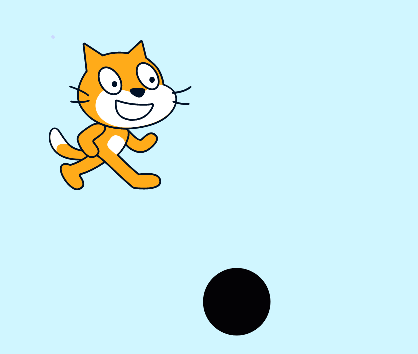
\includegraphics[width=\textwidth]{figure/1-1.png}
                \end{minipage}
                \begin{minipage}[t]{.45\textwidth}
                    \centering
                    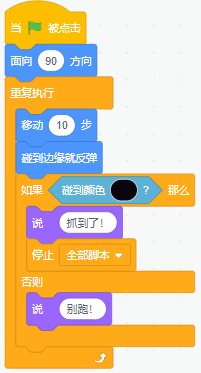
\includegraphics[width=\textwidth]{figure/1-2.png}
                \end{minipage}
                \caption*{第 1 题}
            \end{minipage}
            \begin{minipage}[t]{.4\textwidth}
                \centering
                \begin{minipage}[t]{.36\textwidth}
                    \centering
                    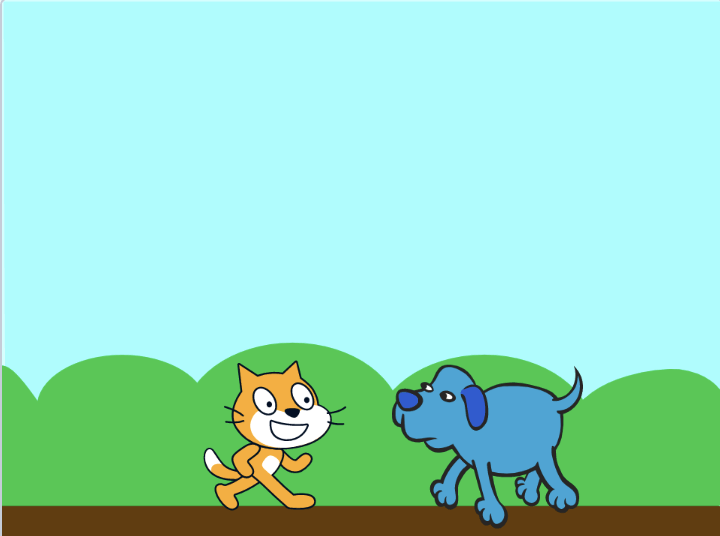
\includegraphics[width=\textwidth]{figure/3-1.png}
                \end{minipage}
                \begin{minipage}[t]{.3\textwidth}
                    \centering
                    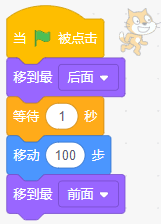
\includegraphics[width=\textwidth]{figure/3-2.png}
                \end{minipage}
                \begin{minipage}[t]{.3\textwidth}
                    \centering
                    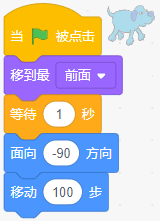
\includegraphics[width=\textwidth]{figure/3-3.png}
                \end{minipage}
                \caption*{第 3 题}
            \end{minipage}
            % \begin{minipage}[t]{.15\textwidth}
            %     \centering
            %     
\includegraphics[width=\textwidth]{figure/2.png}
            %     \caption*{第 2 题}
            % \end{minipage}
            % \begin{minipage}[t]{.16\textwidth}
            %     \centering
            %     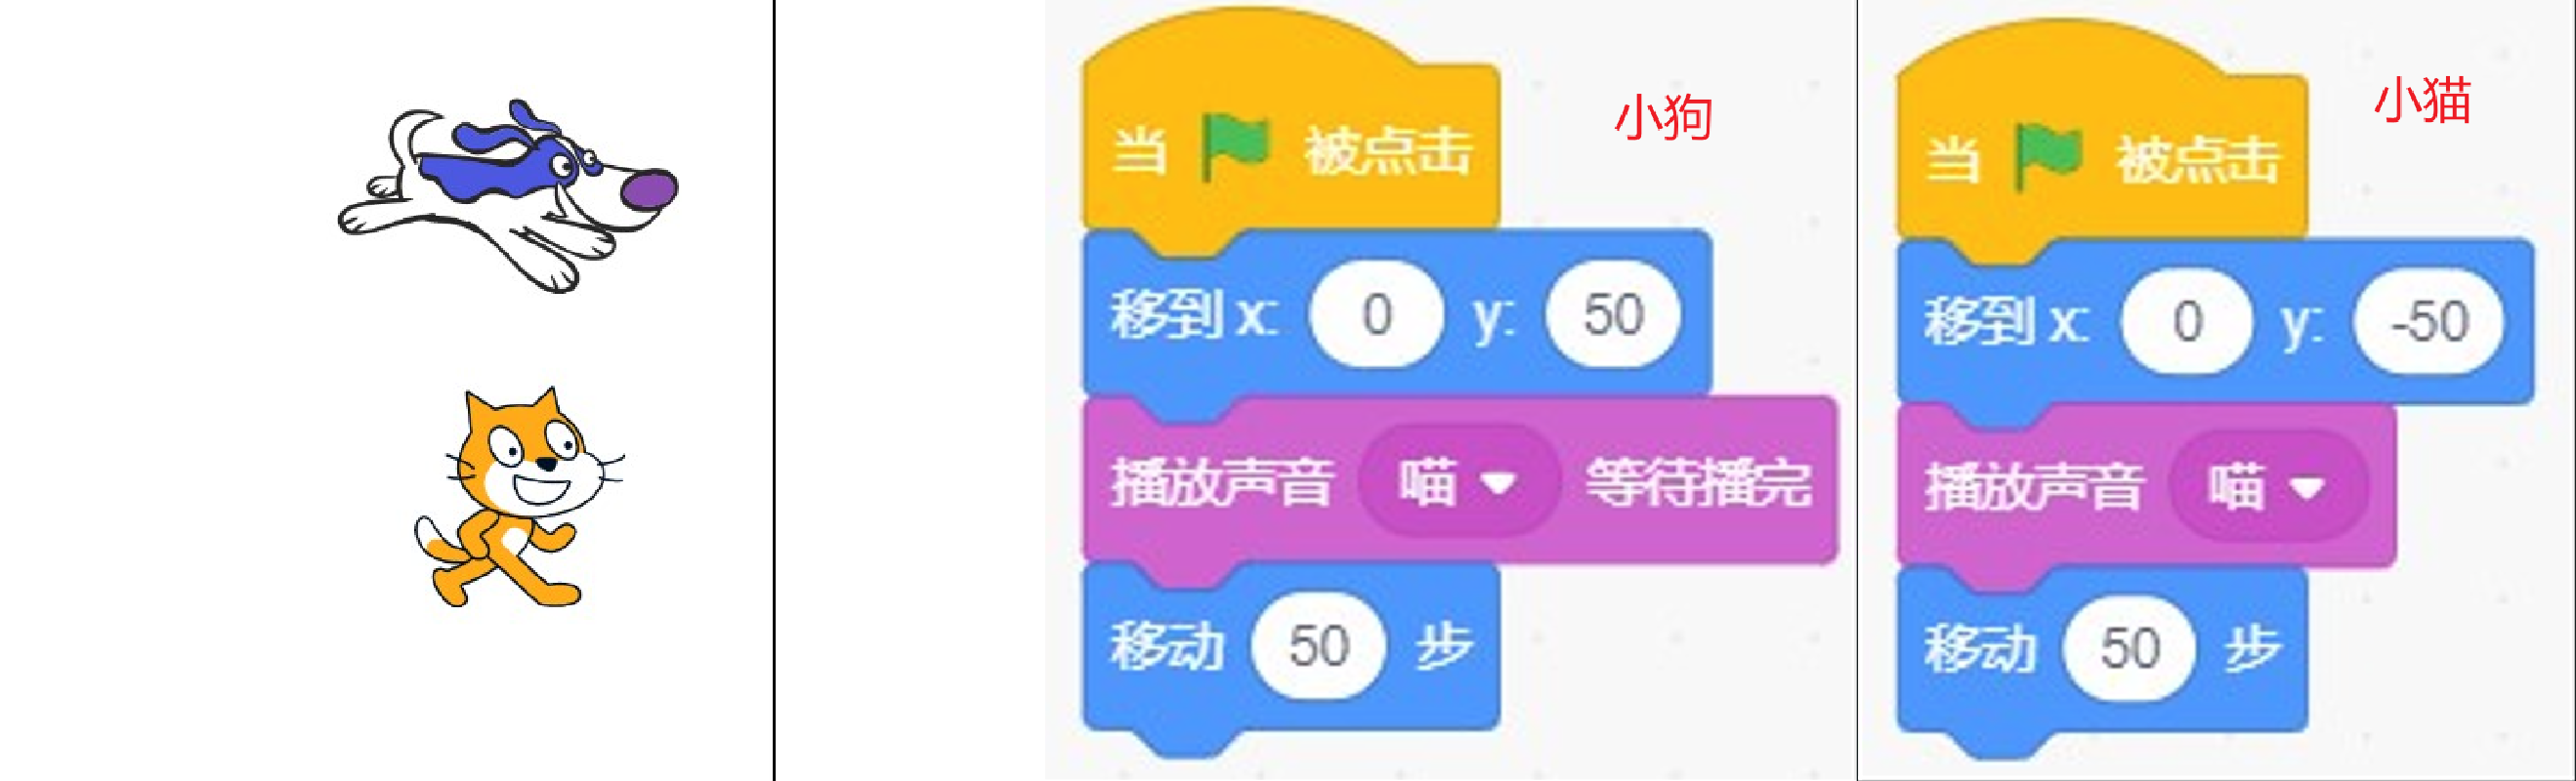
\includegraphics[width=\textwidth]{figure/3.png}
            %     \caption*{第 3 题}
            % \end{minipage}
            % \begin{minipage}[t]{.31\textwidth}
            %     \centering
            %     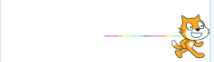
\includegraphics[width=\textwidth]{figure/6.png}
            %     \caption*{第 6 题}
            % \end{minipage}
            % \begin{minipage}[t]{.15\textwidth}
            %     \centering
            %     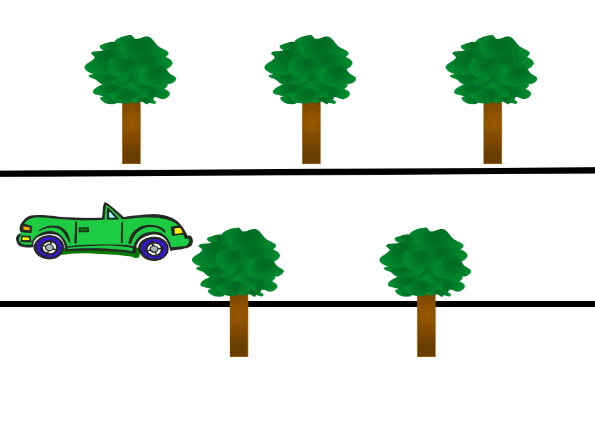
\includegraphics[width=\textwidth]{figure/7.png}
            %     \caption*{第 7 题}
            % \end{minipage}
        \end{figure}

        % 3
        \item 小猫和小狗的初始位置、程序如下图所示。点击绿旗程序运行后,两个角色重叠在一起,程序运行结束后舞台上能看到? \hq
        \begin{tasks}(4)
            \task 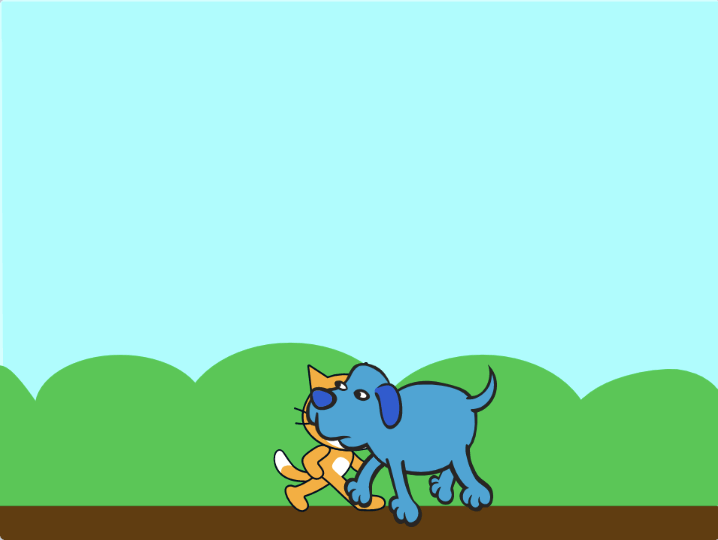
\includegraphics[width=.15\textwidth]{figure/3a.png}
            \task 
\includegraphics[width=.15\textwidth]{figure/3b.png}
            \task 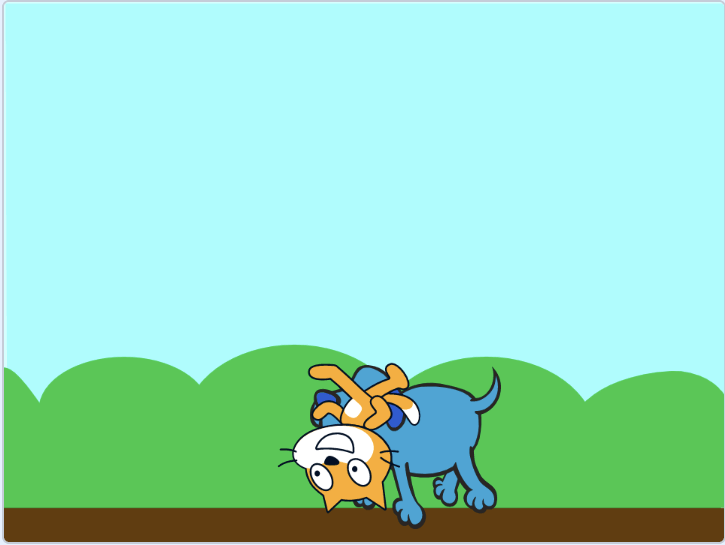
\includegraphics[width=.15\textwidth]{figure/3c.png}
            \task 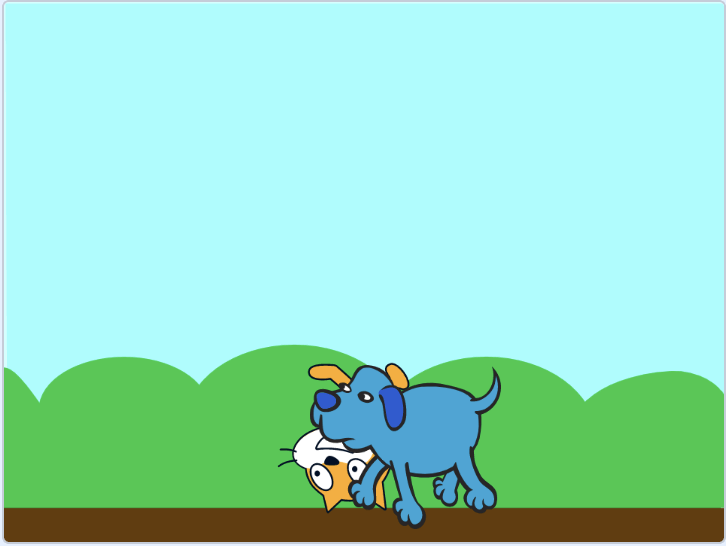
\includegraphics[width=.15\textwidth]{figure/3d.png}
        \end{tasks}

        % 4
        \item 小雨在舞台上使用画笔绘制了一棵圣诞树,他觉得不好看想要重新绘制,可以清除这棵圣诞树的积木是?\hq
        \begin{tasks}(4)
            \task 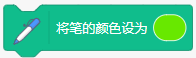
\includegraphics[width=.15\textwidth]{figure/4a.png}
            \task 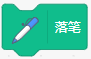
\includegraphics[width=.08\textwidth]{figure/4b.png}
            \task 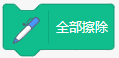
\includegraphics[width=.1\textwidth]{figure/4c.png}
            \task 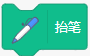
\includegraphics[width=.08\textwidth]{figure/4d.png}
        \end{tasks}

        % 5
        \item 下列哪个选项不是循环语句? \hq
        \begin{tasks}(4)
            \task 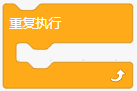
\includegraphics[width=.12\textwidth]{figure/5a.png}
            \task 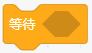
\includegraphics[width=.12\textwidth]{figure/5b.png}
            \task 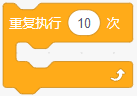
\includegraphics[width=.12\textwidth]{figure/5c.png}
            \task 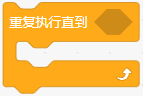
\includegraphics[width=.12\textwidth]{figure/5d.png}
        \end{tasks}

        % 6
        \item 设计一个游戏,小鸟碰到管道游戏失败,程序结束,下列哪个选项可以实现此效果?\hq
        \begin{tasks}(4)
            \task 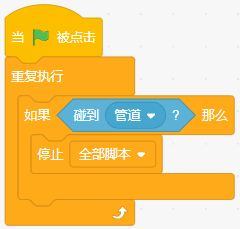
\includegraphics[width=.15\textwidth]{figure/6a.png}
            \task 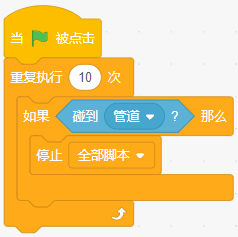
\includegraphics[width=.145\textwidth]{figure/6b.png}
            \task 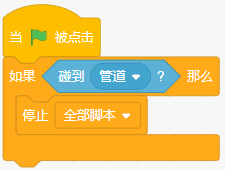
\includegraphics[width=.18\textwidth]{figure/6c.png}
            \task 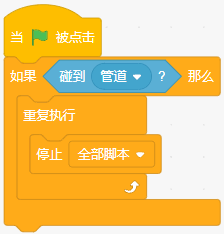
\includegraphics[width=.14\textwidth]{figure/6d.png}
        \end{tasks}

        \newpage
        % 7
        \item 如下图所示,两条黑线中间代表马路,汽车在马路上行驶,下列哪个选项可以检测汽车是否开出了马路?\hq
        \begin{tasks}(4)
            \task 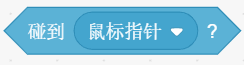
\includegraphics[width=.15\textwidth]{figure/7a.png}
            \task 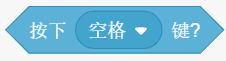
\includegraphics[width=.15\textwidth]{figure/7b.png}
            \task 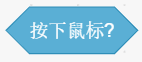
\includegraphics[width=.1\textwidth]{figure/7c.png}
            \task 
\includegraphics[width=.14\textwidth]{figure/7d.png}
        \end{tasks}

        % 8
        \item 请观察下图中已有图形的规律,第一行中间方格和第二行第一个方格分别应填的图形是?\hq
        \begin{tasks}(4)
            \task \tikz \draw (0:0) -- (0:2ex) -- (60:2ex) -- cycle; \tikz \draw (0,0) rectangle (2ex, 2ex);
            \task \tikz \draw (0,0) rectangle (2ex, 2ex); \tikz \draw (0,0) rectangle (2ex, 2ex);
            \task \tikz \draw (0:0) -- (0:2ex) -- (60:2ex) -- cycle; \tikz \draw (0:0) -- (0:2ex) -- (60:2ex) -- cycle;
            \task \tikz \draw (0,0) circle (1ex); \tikz \draw (0:0) -- (0:2ex) -- (60:2ex) -- cycle;
        \end{tasks}

        % 9
        \item 下列说法正确的是?\hq
        \begin{tasks}
            \task 比0小的数都是负数
            \task 如果向上走记为正数,那么向左走记为负数
            \task $A$点的$x$坐标为30,$B$点的$x$坐标为$-10$,这两点间的$x$坐标相差20
            \task 负数相加有可能等于正数
        \end{tasks}

        \begin{figure}[htbp]
            \centering
            \begin{minipage}[t]{.22\textwidth}
                \centering
                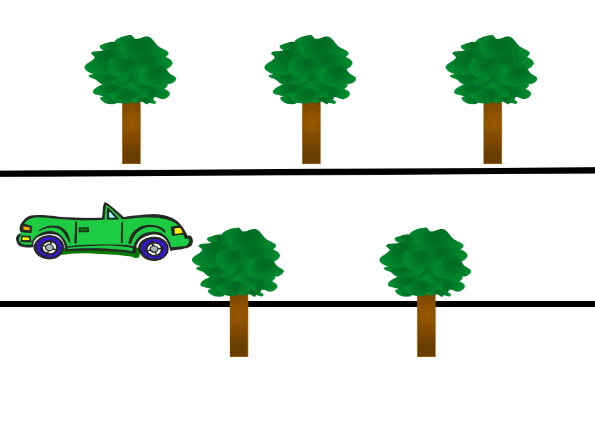
\includegraphics[width=\textwidth]{figure/7.png}
                \caption*{第 7 题}
            \end{minipage}
            \begin{minipage}[t]{.16\textwidth}
                \centering
                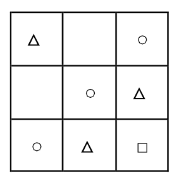
\includegraphics[width=\textwidth]{figure/8.png}
                \caption*{第 8 题}
            \end{minipage}
            \begin{minipage}[t]{.15\textwidth}
                \centering
                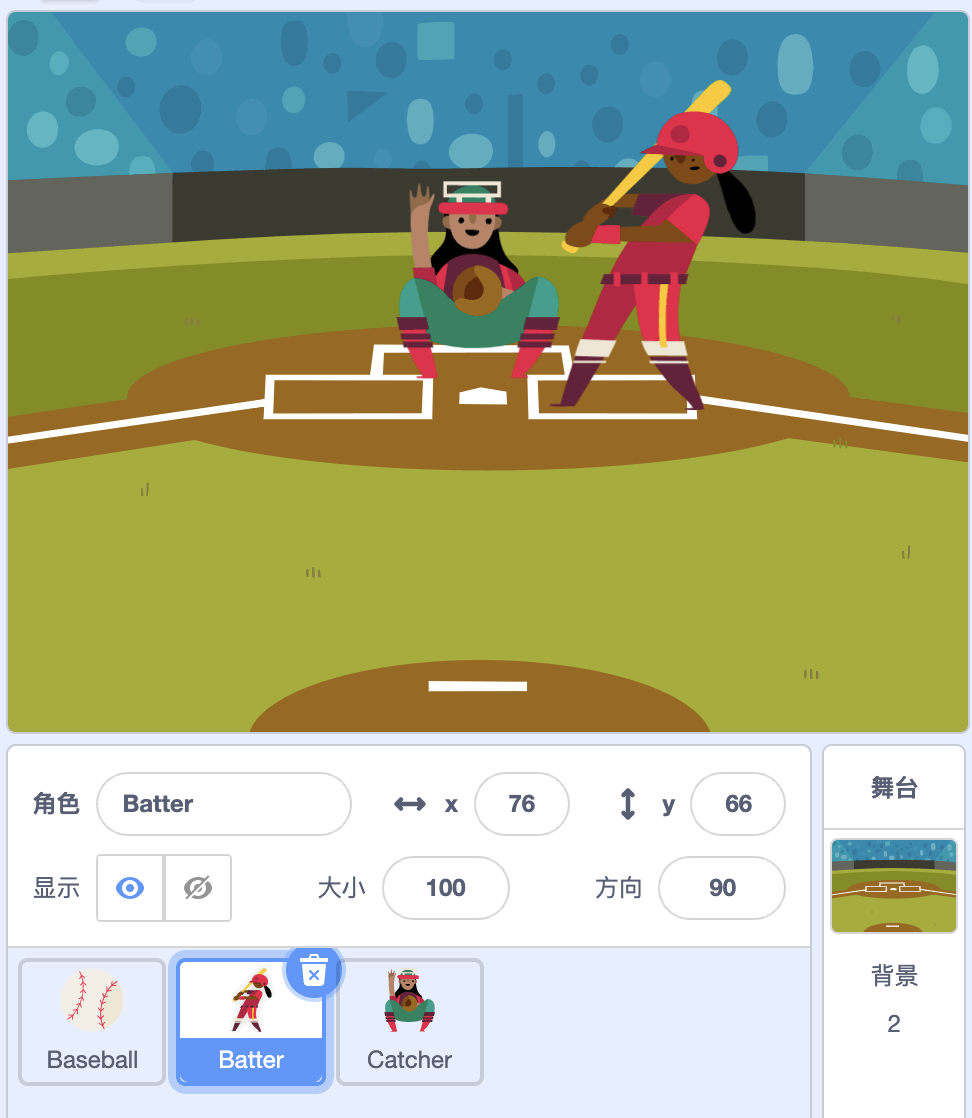
\includegraphics[width=\textwidth]{figure/10.png}
                \caption*{第 10 题}
            \end{minipage}
            \begin{minipage}[t]{.45\textwidth}
                \centering
                \begin{minipage}[t]{.43\textwidth}
                    \centering
                    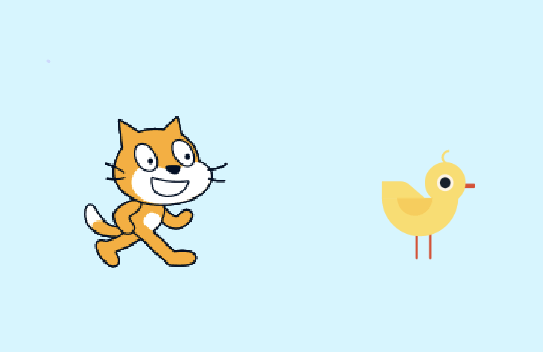
\includegraphics[width=\textwidth]{figure/11-1.png}
                \end{minipage}
                \begin{minipage}[t]{.26\textwidth}
                    \centering
                    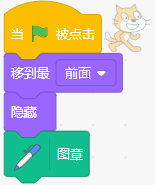
\includegraphics[width=\textwidth]{figure/11-2.png}
                \end{minipage}
                \begin{minipage}[t]{.26\textwidth}
                    \centering
                    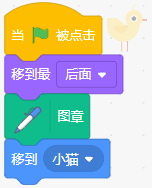
\includegraphics[width=\textwidth]{figure/11-3.png}
                \end{minipage}
                \caption*{第 11 题}
            \end{minipage}
        \end{figure}

        % 10
        \item 棒球游戏的舞台和角色列表如下图所示,请问有几个角色?\hq
        \begin{tasks}(4)
            \task 1个
            \task 2个
            \task 3个
            \task 4个
        \end{tasks}

        % 11
        \item 程序运行前,小猫和小鸡的初始位置如下图所示。点击一次绿旗,舞台上显示?\hq
        \begin{tasks}(4)
            \task 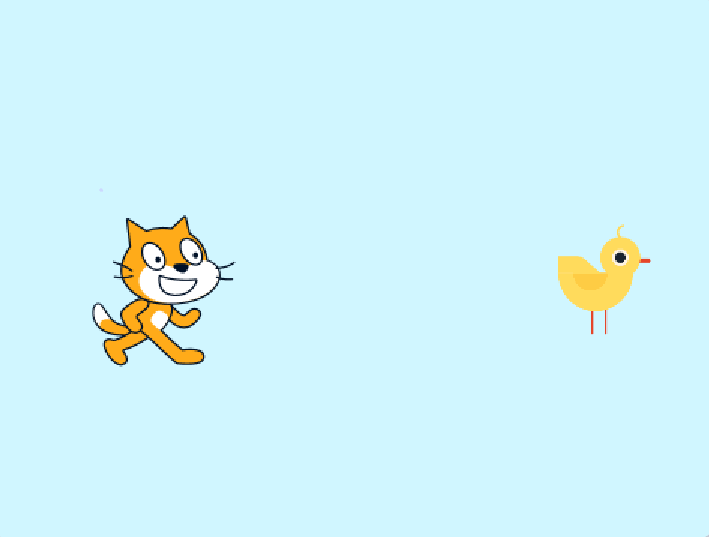
\includegraphics[width=.15\textwidth]{figure/11a.png}
            \task 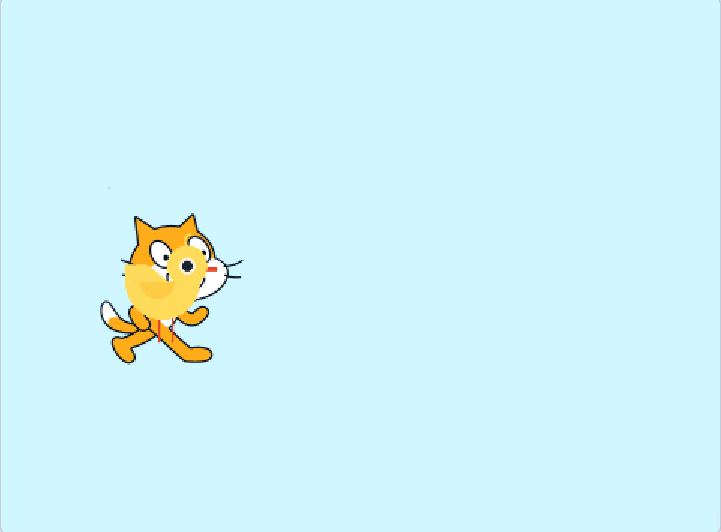
\includegraphics[width=.15\textwidth]{figure/11b.png}
            \task 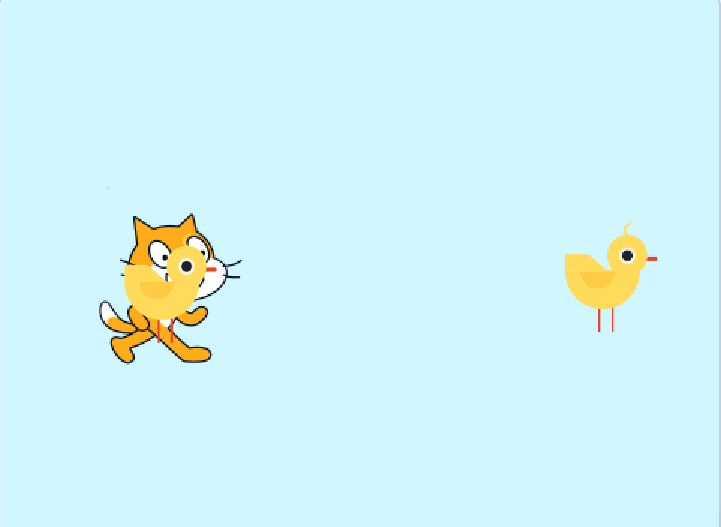
\includegraphics[width=.15\textwidth]{figure/11c.png}
            \task 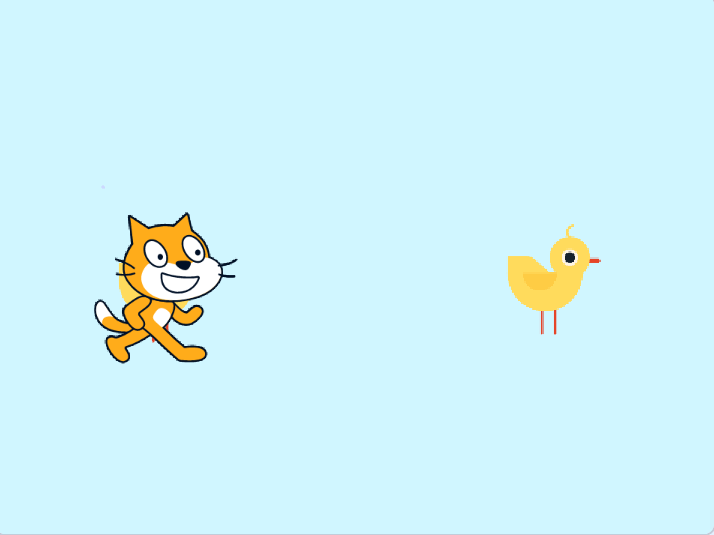
\includegraphics[width=.15\textwidth]{figure/11d.png}
        \end{tasks}

        % 12
        \item 小猫和香蕉的位置、程序如下图所示。点击绿旗,下列说法正确的是?\hq
        \begin{tasks}
            \task 点击绿旗后,小猫说1次“我碰到香蕉啦!”2秒后,说话框消失
            \task 点击绿旗后,小猫说会一直说“我碰到香蕉啦!”,并且说话框不消失
            \task 点击绿旗后,香蕉消失了,小猫不会说“我碰到香蕉啦!”
            \task 点击绿旗后,小猫说1次“我碰到香蕉啦!”2秒后,说话框消失并且香蕉也跟着消失了
        \end{tasks}

        \begin{minipage}[t]{.21\textwidth}
            \centering
            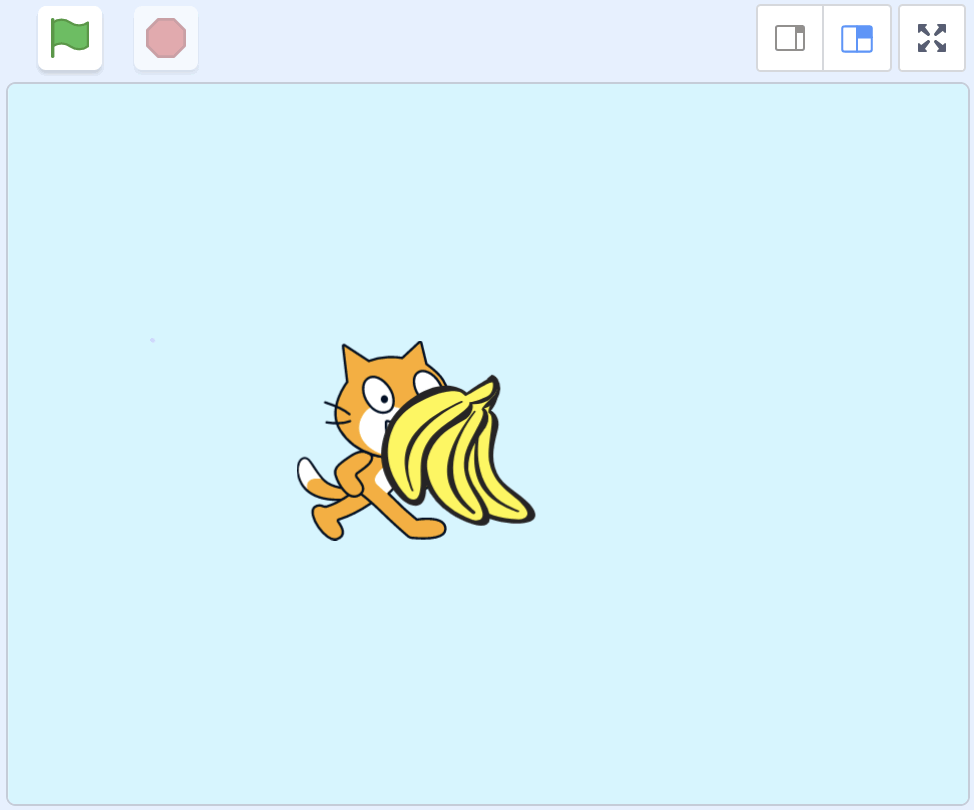
\includegraphics[width=\textwidth]{figure/12-1.png}
        \end{minipage}
        \begin{minipage}[t]{.22\textwidth}
            \centering
            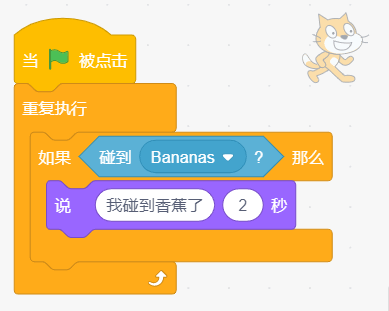
\includegraphics[width=\textwidth]{figure/12-2.png}
        \end{minipage}
        \begin{minipage}[t]{.26\textwidth}
            \centering
            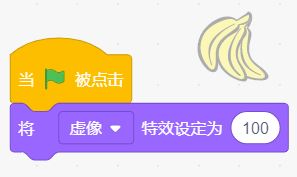
\includegraphics[width=\textwidth]{figure/12-3.png}
        \end{minipage}

        \newpage
        % 13
        \item 演员的程序如下图所示,下列哪一个场景在程序运行后,演员不能说:“唱歌”的是?\hq
        \begin{tasks}(4)
            \task 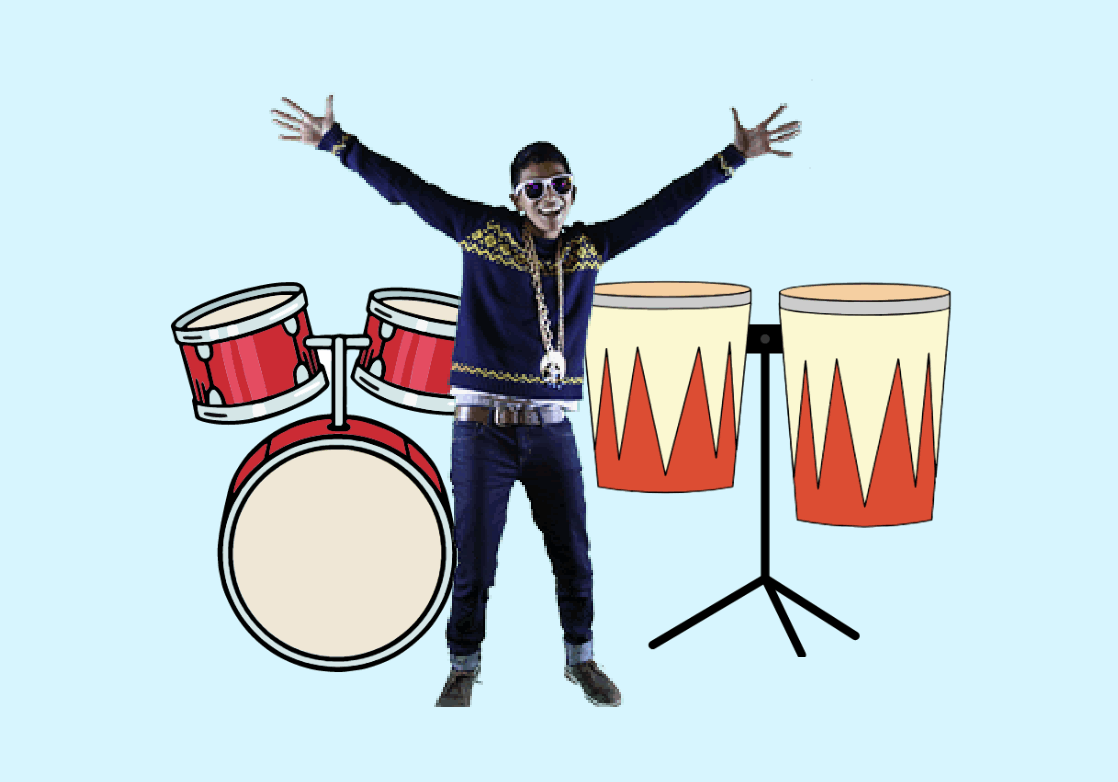
\includegraphics[width=.15\textwidth]{figure/13a.png}
            \task 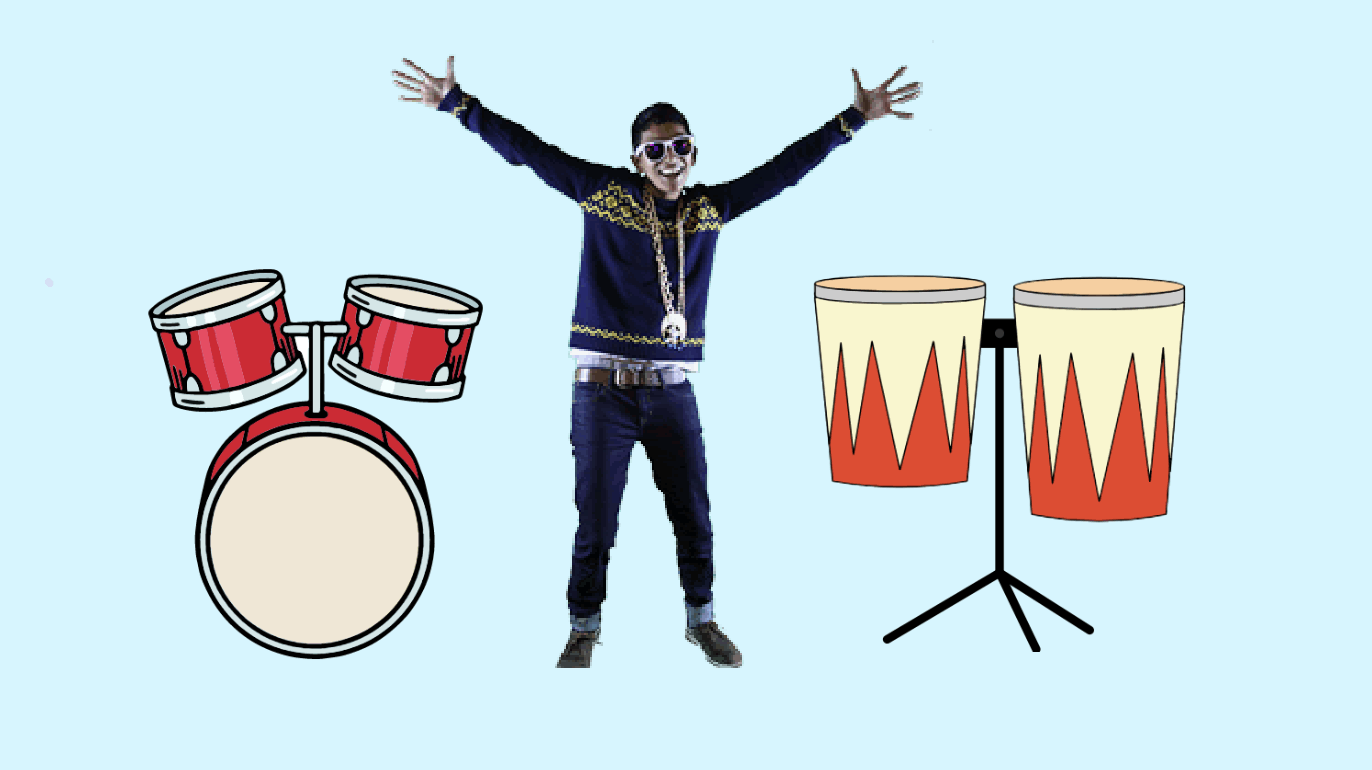
\includegraphics[width=.18\textwidth]{figure/13b.png}
            \task 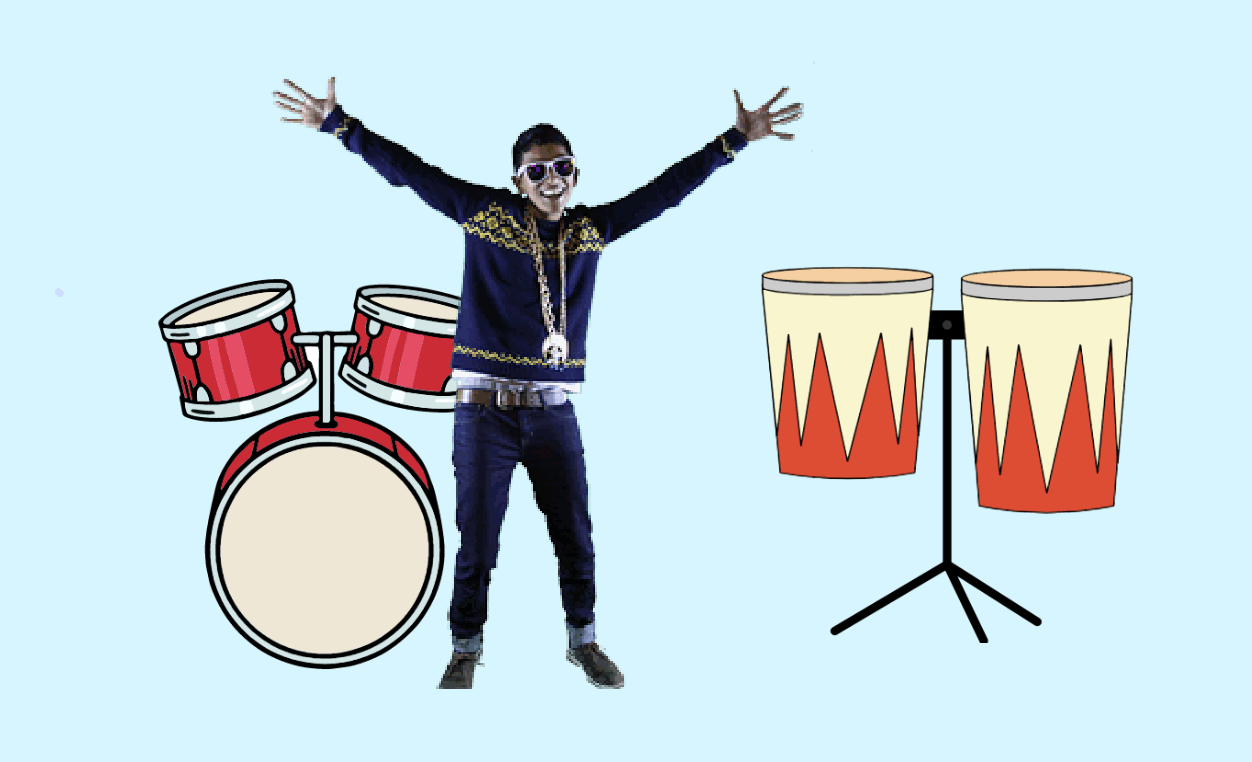
\includegraphics[width=.17\textwidth]{figure/13c.png}
            \task 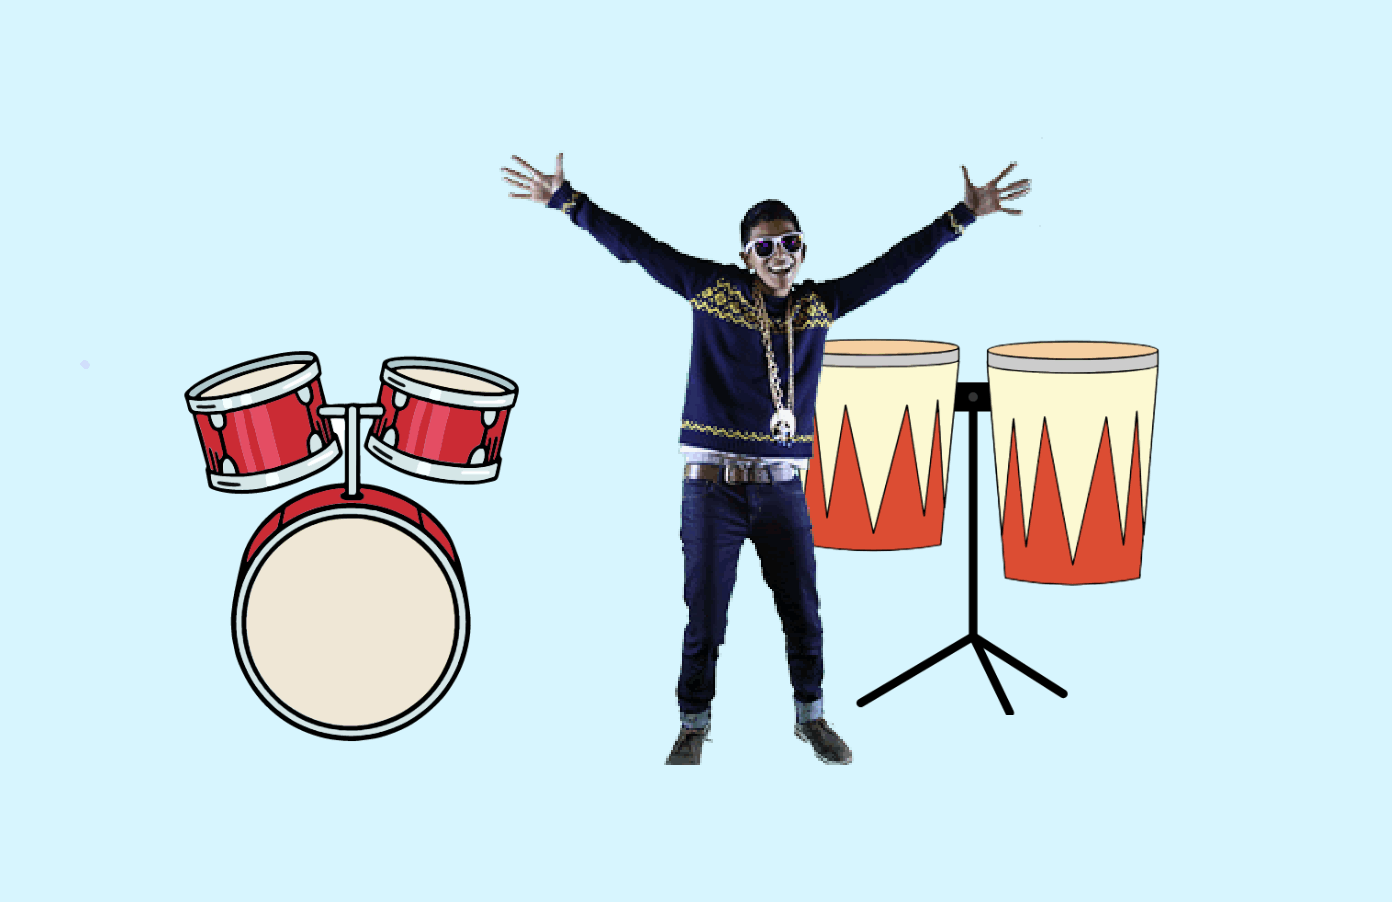
\includegraphics[width=.16\textwidth]{figure/13d.png}
        \end{tasks}
        
        % 14
        \item 运行下图所示程序,角色会依次说出哪几个单词?\hq
        \begin{tasks}(4)
            \task apple\ banana\ orange
            \task banana\ apple\ orange
            \task banana\ orange
            \task banana\ apple
        \end{tasks}

        \begin{figure}[htbp]
            \centering
            \begin{minipage}[t]{.23\textwidth}
                \centering
                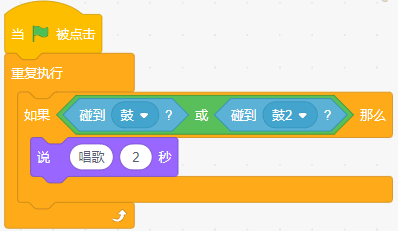
\includegraphics[width=\textwidth]{figure/13.png}
                \caption*{第 13 题}
            \end{minipage}
            \begin{minipage}[t]{.25\textwidth}
                \centering
                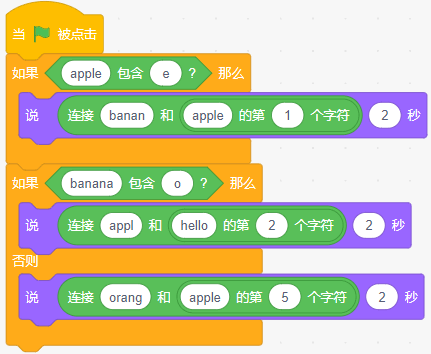
\includegraphics[width=\textwidth]{figure/14.png}
                \caption*{第 14 题}
            \end{minipage}
            \begin{minipage}[t]{.2\textwidth}
                \centering
                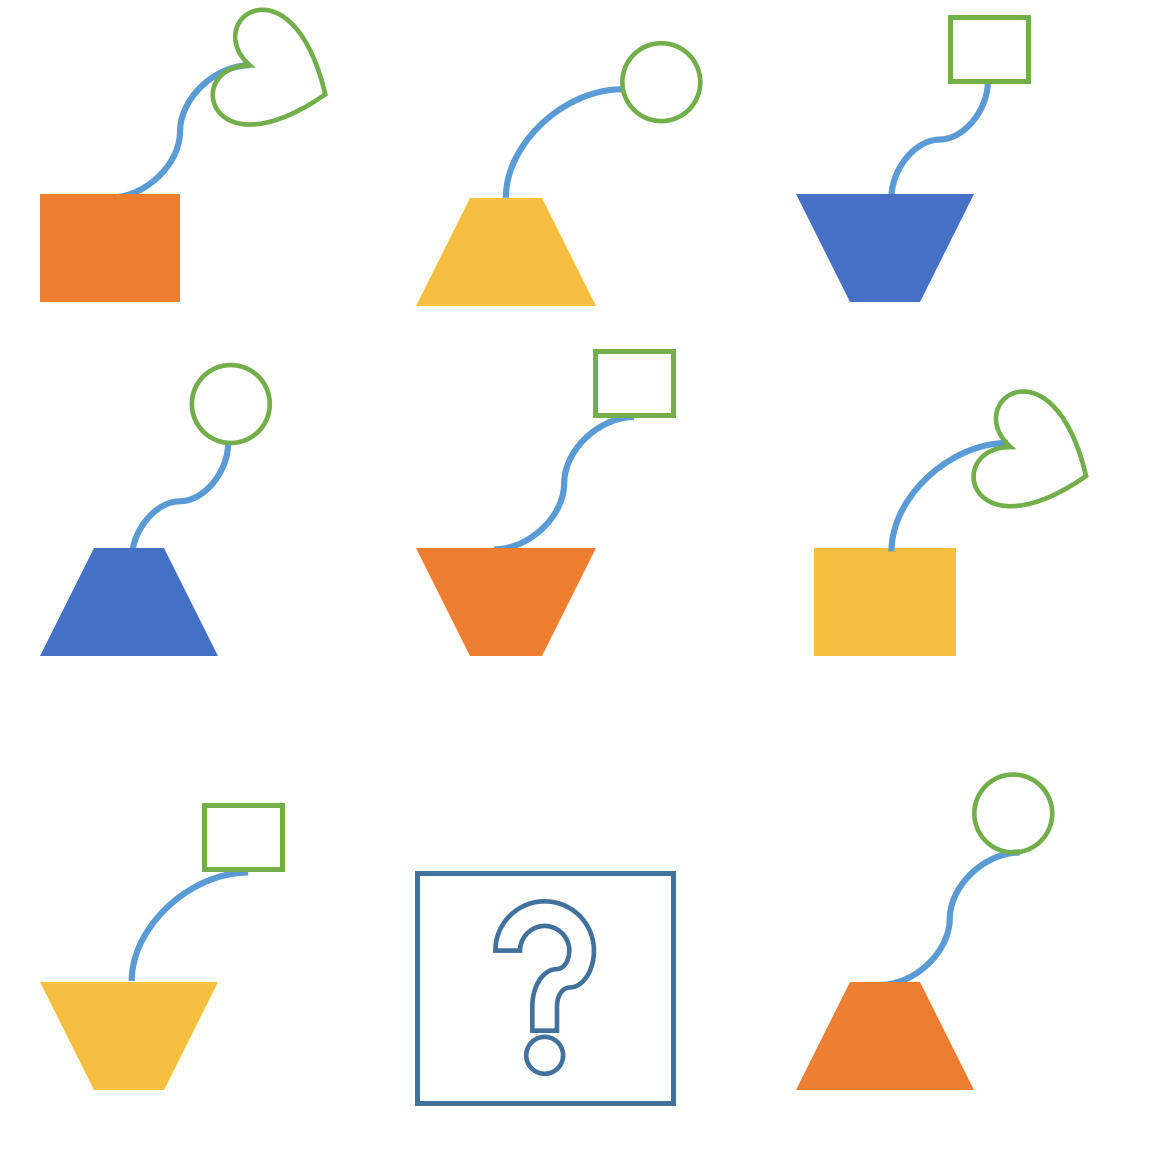
\includegraphics[width=\textwidth]{figure/18.png}
                \caption*{第 18 题}
            \end{minipage}
            \begin{minipage}[t]{.15\textwidth}
                \centering
                \includegraphics[width=\textwidth]{figure/20.png}
                \caption*{第 20 题}
            \end{minipage}
        \end{figure}

        % 15
        \item 下列哪个选项的运行结果是true?\hq
        \begin{tasks}(4)
            \task \includegraphics[width=.16\textwidth]{figure/15a.png}
            \task \includegraphics[width=.16\textwidth]{figure/15b.png}
            \task \includegraphics[width=.18\textwidth]{figure/15c.png}
            \task \includegraphics[width=.18\textwidth]{figure/15d.png}
        \end{tasks}

        % 16
        \item 使用下面哪个选项的工具可以将声音波形从图1变成图2?\hq
        
        \begin{minipage}{.2\textwidth}
            \centering
            \includegraphics[width=\textwidth]{figure/16-1.png}
        \end{minipage}
        \begin{minipage}{.2\textwidth}
            \centering
            \includegraphics[width=\textwidth]{figure/16-2.png}
        \end{minipage}
        \begin{minipage}{.53\textwidth}
            \begin{tasks}(4)
                \task \includegraphics[width=.1\textwidth]{figure/16a.png}
                \task \includegraphics[width=.1\textwidth]{figure/16b.png}
                \task \includegraphics[width=.1\textwidth]{figure/16c.png}
                \task \includegraphics[width=.1\textwidth]{figure/16d.png}
            \end{tasks}
        \end{minipage}

        % 17
        \item 角色和背景的程序如上图所示,其中recording1的长度是6秒,recording2的长度是3秒。点击绿旗运行程序后,下列说法正确的是?\hq
        
        \begin{minipage}{.2\textwidth}
            \centering
            \includegraphics[width=\textwidth]{figure/17-1.png}
        \end{minipage}
        \begin{minipage}{.2\textwidth}
            \centering
            \includegraphics[width=\textwidth]{figure/17-2.png}
        \end{minipage}
        \begin{minipage}{.53\textwidth}
            \begin{tasks}
                \task 角色的声音大小会被舞台的程序设置为 $50\%$
                \task 舞台的声音大小会被角色的程序设置为 $70\%$
                \task 背景的声音先播放完毕,3秒后角色的声音才播放完
                \task 背景的声音播放完毕后,角色的声音也会被停止
            \end{tasks}
        \end{minipage}

        % 18
        \item 观察下图,找出规律。在问号处应该填入哪一个图形?\hq
        \begin{tasks}(4)
            \task \includegraphics[width=.08\textwidth]{figure/18a.png}
            \task \includegraphics[width=.08\textwidth]{figure/18b.png}
            \task \includegraphics[width=.08\textwidth]{figure/18c.png}
            \task \includegraphics[width=.08\textwidth]{figure/18d.png}
        \end{tasks}

        % 19
        \item 甲、乙、丙、丁四名学生猜数学成绩: 甲说:如果我得优,那么乙也得优 乙说:如果我得优,那么丙也得优 丙说:如果我得优,那么丁也得优 结果大家说的都没错,但是只有两个人得了优,请问得优的是那两位同学?\hq
        \begin{tasks}(4)
            \task 甲、乙
            \task 丙、丁
            \task 甲、丁
            \task 乙、丁
        \end{tasks}

        % 20
        \item 默认小猫角色,白色背景,点击绿旗运行程序后,舞台上出现的图案是?\hq
        \begin{tasks}(4)
            \task \includegraphics[width=.15\textwidth]{figure/20a.png}
            \task \includegraphics[width=.15\textwidth]{figure/20b.png}
            \task \includegraphics[width=.15\textwidth]{figure/20c.png}
            \task \includegraphics[width=.15\textwidth]{figure/20d.png}
        \end{tasks}

        % 21
        \item 小猫角色程序如下图所示,一直按住空格键并点击绿旗,舞台上会出现什么效果?\hq
        \begin{tasks}(2)
            \task 小猫一直向右转
            \task 小猫一直向左转
            \task 小猫停止转动
            \task 能够明显看出小猫先向右转,再向左转
        \end{tasks}

        % 22
        \item 小鱼的初始位置和程序如下图所示,点击绿旗后,下列说法正确的是? \hq
        
        \begin{minipage}{.18\textwidth}
            \centering
            \includegraphics[width=\textwidth]{figure/22-1.png}
        \end{minipage}
        \begin{minipage}{.13\textwidth}
            \centering
            \includegraphics[width=\textwidth]{figure/22-2.png}
        \end{minipage}
        \begin{minipage}{.63\textwidth}
            \begin{tasks}
                \task 小鱼一直向右移动,直到舞台边缘停止
                \task 按下“→”键,小鱼向右移动;松开“→”键,小鱼向左移动
                \task 按下“→”键,小鱼向右移动;松开“→”键,小鱼向右移动
                \task 小鱼一动不动
            \end{tasks}
        \end{minipage}

        % 23
        \item 下列哪段程序是根据如下流程图编写出来的?\hq
        \begin{tasks}(4)
            \task \includegraphics[width=.18\textwidth]{figure/23a.png}
            \task \includegraphics[width=.15\textwidth]{figure/23b.png}
            \task \includegraphics[width=.14\textwidth]{figure/23c.png}
            \task \includegraphics[width=.15\textwidth]{figure/23d.png}
        \end{tasks}

        \begin{figure}[htbp]
            \centering
            \begin{minipage}[t]{.18\textwidth}
                \centering
                \includegraphics[width=\textwidth]{figure/21.png}
                \caption*{第 21 题}
            \end{minipage}
            \begin{minipage}[t]{.14\textwidth}
                \includegraphics[width=\textwidth]{figure/23.png}
                \caption*{第 23 题}
            \end{minipage}
            \begin{minipage}[t]{.46\textwidth}
                \centering
                \begin{minipage}[t]{.55\textwidth}
                    \centering
                    \includegraphics[width=\textwidth]{figure/24-1.png}
                \end{minipage}
                \begin{minipage}[t]{.35\textwidth}
                    \centering
                    \includegraphics[width=\textwidth]{figure/24-2.png}
                \end{minipage}
                \caption*{第 24 题}
            \end{minipage}
            \begin{minipage}[t]{.155\textwidth}
                \includegraphics[width=\textwidth]{figure/25.png}
                \caption*{第 25 题}
            \end{minipage}
        \end{figure}

        % 24
        \item 角色的初始位置和飞船的程序如下图所示。点击绿旗后,不会出现的效果是?\hq
        \begin{tasks}(2)
            \task 程序运行完后,飞船的角度为180度
            \task 飞船先向右转,然后再向右移动
            \task 飞船碰到“Crystal”后,仍继续向右移动
            \task 飞船最后一个动作是说“遇到阻碍,无法前行。”
        \end{tasks}

        % 25
        \item 气球角色的程序如下图所示,分别在位置 \ding{172} 和位置 \ding{173} 填入哪个选项才能让气球的大小最后变为100。\hq
        \begin{tasks}(4)
            \task 3, 8
            \task 6, 2
            \task 4, 5
            \task 6, 3
        \end{tasks}
    \end{enumerate}

    \newpage
    % 判断题
    {\noindent\textbf{第二部分、判断题(共 10 题,每题 2 分,共20分.)}}
    \begin{enumerate}
        \setcounter{enumi}{25}
        % 26
        \item 执行完这段程序后,可以在舞台上画出一个正方形。\hq

        % 27
        \item 默认小猫角色,执行完下图程序后,最终会滑行到$(x:100,y:0)$的位置。\hq
        
        \begin{figure}[htbp]
            \centering
            \begin{minipage}[t]{.13\textwidth}
                \centering
                \includegraphics[width=\textwidth]{figure/26.png}
                \caption*{第 26 题}
            \end{minipage}
            \begin{minipage}[t]{.26\textwidth}
                \centering
                \includegraphics[width=\textwidth]{figure/27.png}
                \caption*{第 27 题}
            \end{minipage}
            \begin{minipage}[t]{.15\textwidth}
                \centering
                \includegraphics[width=\textwidth]{figure/31.png}
                \caption*{第 31 题}
            \end{minipage}
            \begin{minipage}[t]{.35\textwidth}
                \centering
                \begin{minipage}[t]{.3\textwidth}
                    \centering
                    \includegraphics[width=\textwidth]{figure/32-1.png}
                \end{minipage}
                \begin{minipage}[t]{.3\textwidth}
                    \centering
                    \includegraphics[width=\textwidth]{figure/32-2.png}
                \end{minipage}
                \begin{minipage}[t]{.3\textwidth}
                    \centering
                    \includegraphics[width=\textwidth]{figure/32-3.png}
                \end{minipage}
                \caption*{第 32 题}
            \end{minipage}
        \end{figure}

        % 28
        \item 最先添加的角色出现在舞台的最上层,最后添加的角色出现在舞台的最下层。\hq

        % 29
        \item 如图\includegraphics[width=.12\textwidth]{figure/29.png}积木只能判断是否碰到其他角色和鼠标指针,不能判断是否碰到舞台边缘。\hq

        % 30
        \item 默认小猫角色,运行\includegraphics[width=.2\textwidth]{figure/30.png}程序后,小猫会说:“3” 。\hq

        % 31
        \item 只能通过声音标签下的录制按钮录制声音。\hq

        % 32
        \item 有\ding{172} \ding{173} \ding{174} \ding{175} 四个小球如上图所示,最轻的小球是\ding{173}。\hq

        % 33
        \item 编写一个游戏,猴子碰到障碍物,向后移动,否则就向前移动。可以用下列积木来实现这个功能。\hq
        
        \begin{figure}[htbp]
            \centering
            \begin{minipage}[t]{.13\textwidth}
                \centering
                \includegraphics[width=\textwidth]{figure/33.png}
                \caption*{第 33 题}
            \end{minipage}
            \begin{minipage}[t]{.36\textwidth}
                \centering
                \begin{minipage}[t]{.4\textwidth}
                    \centering
                    \includegraphics[width=\textwidth]{figure/34-1.png}
                \end{minipage}
                \begin{minipage}[t]{.52\textwidth}
                    \centering
                    \includegraphics[width=\textwidth]{figure/34-2.png}
                \end{minipage}
                \caption*{第 34 题}
            \end{minipage}
            \begin{minipage}[t]{.1\textwidth}
                \centering
                \includegraphics[width=\textwidth]{figure/35.png}
                \caption*{第 35 题}
            \end{minipage}
        \end{figure}

        % 34
        \item 敌方飞机的程序如上图所示,两段程序都能实现,碰到我方飞机时,游戏结束。\hq

        % 35
        \item 执行上图程序,角色能够向前移动100步,并且一直切换造型。\hq
    \end{enumerate}

    \newpage
    {\noindent \textbf{第三部分、编程题(共 2 题,共30分.)}}
    \begin{enumerate}
        \setcounter{enumi}{35}
        
        % 36
        \item 猫捉老鼠:
        
        1. 准备工作
        \begin{tasks}[label = (\arabic*)]
            \task 删除默认小猫角色,从角色库中添加Cat2、Mouse1、Bread角色;
            \task 从背景库添加Blue Sky2背景,并复制出两个相同的背景,分别添加文字“win”和“lose"。
        \end{tasks}
        2. 功能实现
        \begin{tasks}[label = (\arabic*)]
            \task 程序开始,背景、角色的初始位置下图所示;
            \task 当绿旗被点击,面包移到随机位置,老鼠面向面包方向,一直向前移动;
            \task 当绿旗被点击,每次按下鼠标,小猫面向鼠标指针方向,移动10步;
            \task 当面包碰到老鼠,换成“lose”背景并停止所有程序;
            \task 当小猫碰到老鼠,换成“win”背景并停止所有程序。
        \end{tasks}
        \begin{figure}[htbp]
            \centering
            \begin{minipage}[t]{.29\textwidth}
                \centering
                \includegraphics[width=\textwidth]{figure/36-1.png}
            \end{minipage}
            \begin{minipage}[t]{.29\textwidth}
                \centering
                \includegraphics[width=\textwidth]{figure/36-2.png}
            \end{minipage}
            \begin{minipage}[t]{.29\textwidth}
                \centering
                \includegraphics[width=\textwidth]{figure/36-3.png}
            \end{minipage}
        \end{figure}

        %37
        \item 电子画板:
        
        1. 准备工作
        \begin{tasks}[label = (\arabic*)]
            \task 删除默认的小猫角色,保留默认白色背景;
            \task 从角色库添加Arrow1角色作为画笔;
            \task 绘制五个角色:颜色分别为红、黄、绿、蓝、紫的圆形;
            \task 将Arrow1角色的第一个造型修改为下图所示状态,箭头尖端在角色中心位置。
        \end{tasks}
        2. 功能实现
        \begin{tasks}[label = (\arabic*)]
            \task 点击绿旗,Arrow1跟随鼠标指针移动;
            \task 按下鼠标能够让画笔落笔,松开鼠标能让画笔抬笔;
            \task Arrow1每碰到一个圆形角色(注意不是碰到颜色),就将画笔的颜色设置为该角色对应的颜色;
        \end{tasks}

        \begin{figure}[htbp]
            \centering
            \begin{minipage}[t]{.29\textwidth}
                \centering
                \includegraphics[width=\textwidth]{figure/37-1.png}
            \end{minipage}
            \begin{minipage}[t]{.29\textwidth}
                \centering
                \includegraphics[width=\textwidth]{figure/37-2.png}
            \end{minipage}
        \end{figure}
    \end{enumerate}
\end{document}